\documentclass[12pt,a4paper]{report}

\usepackage{graphicx}
\usepackage{amsmath}
\usepackage{setspace}
\usepackage{geometry}
\usepackage{float}
\usepackage{hyperref}
\usepackage{titlesec}

\hypersetup{hidelinks}

\geometry{margin=1in}

% ===== SPACING FIX =====
\onehalfspacing
\raggedbottom

% ===== CHAPTER GAP FIX (MAIN FIX) =====
\titleformat{\chapter}[display]
  {\normalfont\huge\bfseries}
  {\chaptername\ \thechapter}
  {10pt}
  {\Huge}

\titlespacing*{\chapter}{0pt}{0pt}{20pt}

% ===== FORCE REMOVE ANY EXTRA SPACE =====
\makeatletter
\def\@makechapterhead#1{%
  \vspace*{0pt}
  {\parindent \z@ \raggedright \normalfont
    \huge\bfseries \chaptername\ \thechapter\par\nobreak
    \vskip 10pt
    \Huge #1\par\nobreak
    \vskip 20pt
  }}
\makeatother
\begin{document}

%================ TITLE PAGE =================%
\begin{titlepage}
\centering

{\Huge \textbf{Hybrid CPU–GPU Based Real-Time Crowd Simulation}}\\[0.5cm]

{\Large A Project Component for}\\
{\Large \textbf{Parallel and Distributed Computing (UCS645)}}\\[1.5cm]

\textbf{By}\\[0.5cm]

\begin{tabular}{ll}
1. Narhar Singh & 102483046 \\
2. Raghav Jain & 102483049 \\
3. Harkirat Singh  & 102317074 \\
\end{tabular}

\vspace{1.5cm}

\textbf{Under the guidance of}\\
Dr. Saif Nalband\\
(Assistant Professor, DCSE)\\
\begin{figure}[h]
\centering
\includegraphics[width=70mm, height=40mm]{"tietlogo.jpg"}
\label{fig:images}
\end{figure}

DEPARTMENT OF COMPUTER SCIENCE AND ENGINEERING\\
THAPAR INSTITUTE OF ENGINEERING AND TECHNOLOGY\\
(Deemed to be University)\\
PATIALA - 147004\\[1cm]

\textbf{April, 2026}

\end{titlepage}

\tableofcontents
\newpage

%================ INTRODUCTION =================%
\chapter{Introduction}

\section{Background}

The simulation of crowd dynamics is a fundamental problem in computational science with wide-ranging applications in pedestrian flow analysis, evacuation planning, swarm robotics, and intelligent transportation systems. These simulations aim to replicate realistic human movement patterns by modeling individuals as autonomous agents interacting with their environment.

A key challenge in such simulations arises from the computational complexity associated with agent interactions. Each agent must continuously evaluate its surroundings and adjust its behavior accordingly, leading to an overall computational complexity that grows quadratically with the number of agents.

Traditional CPU-based implementations struggle to maintain real-time performance under such conditions. This limitation necessitates the adoption of parallel computing paradigms capable of handling large-scale simulations efficiently.

\section{Introduction to Problem Statement}

The primary problem addressed in this work is the development of a scalable and efficient simulation framework capable of handling thousands of agents in real time. Each agent must:
\begin{itemize}
\item Navigate towards designated exit points
\item Avoid collisions with other agents and obstacles
\item Exhibit realistic crowd behavior

\end{itemize}
\begin{figure}[H]
\centering
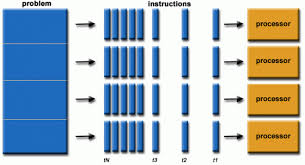
\includegraphics[width=0.8\textwidth]{Figure1.jpeg}
\caption{Conceptual Representation of CPU vs GPU Parallel Processing}
\end{figure}

The challenge lies in balancing computational efficiency with behavioral realism. To address this, a hybrid CPU--GPU architecture is proposed, wherein computationally intensive tasks are offloaded to the GPU.

As highlighted in the template, GPUs follow a throughput-oriented design philosophy, enabling massive parallel execution, unlike CPUs which are optimized for low-latency sequential processing.

%================ LITERATURE REVIEW =================%
\chapter{Literature Review}

The Boids model, introduced by Reynolds (1987), forms the foundation of most crowd simulation systems. It models collective behavior using three fundamental rules: separation, alignment, and cohesion.

Subsequent research has explored optimization techniques for scaling such simulations. GPU-based implementations using CUDA have demonstrated significant improvements in performance by parallelizing agent updates.

However, many existing systems either lack real-time responsiveness or fail to integrate efficient hybrid architectures combining CPU and GPU capabilities.

\begin{table}[h]
\centering
\caption{Summary of Literature Review}
\begin{tabular}{|c|c|c|c|}
\hline
Reference & Approach & Contribution & Limitation \\
\hline
Reynolds (1987) & Boids Model & Emergent behavior & Not scalable \\
\hline
CUDA Research & GPU Parallelism & High speedup & Memory overhead \\
\hline
Agent Systems & Crowd Modeling & Realistic simulation & High complexity \\
\hline
\end{tabular}
\end{table}

%================ RESEARCH GAPS =================%
\chapter{Research Gaps}

Despite notable advancements in crowd simulation techniques, several limitations persist that directly affect the efficiency and realism of large-scale evacuation systems. One of the primary challenges lies in the limited scalability of traditional CPU-based implementations. Most existing models rely on sequential processing, which becomes increasingly inefficient as the number of agents grows. In dense crowd scenarios, particularly near exits where bottlenecks occur, the computational load increases significantly due to the need for continuous interaction calculations between agents. This makes it difficult to achieve real-time performance using conventional approaches.

Another important gap is related to the underutilization of GPU resources in many existing systems. Although GPU-based methods have been explored, they often suffer from inefficient memory usage, thread divergence, and excessive data transfer between CPU and GPU. Additionally, many models fail to balance computational efficiency with behavioral realism, limiting their ability to simulate phenomena such as congestion, lane formation, and density variations effectively. These challenges highlight the need for a hybrid CPU–GPU approach that can efficiently manage large-scale simulations while maintaining realistic crowd behavior, which is the focus of this project.

%================ PROBLEM FORMULATION =================%
\chapter{Problem Formulation}

The system models a set of $N$ agents in a bounded 2D environment. The primary computational challenge involves calculating the motion of each agent, which is governed by interaction forces derived from all neighboring agents.

\section{The Interaction Model}

The total resultant force acting on a specific agent is defined by the summation of forces exerted by every other agent in the simulation. This is expressed by the formula:

\begin{equation}
F_i = \sum_{j=1}^{N} f(d_{ij})
\end{equation}

where:

\begin{itemize}
    \item $F_i$: Represents the resultant force vector on agent $i$.
    
    \item $d_{ij}$: Denotes the Euclidean distance between agent $i$ and agent $j$.
    
    \item $f(d_{ij})$: Is the interaction function (in this project, it represents the separation force used to prevent collisions).
\end{itemize}

\section{Computational Complexity}

In a traditional sequential environment, calculating these forces for $N$ agents requires $O(N^2)$ operations. As the population scales from 100 to 20{,}000 agents, the computational load becomes too heavy for a standard CPU to process in real time.

\section{Objective}

The core objective of this formulation is to offload these $O(N^2)$ interaction calculations to the GPU. By using parallel processing, these forces are computed for all agents simultaneously, bypassing the sequential bottleneck and maintaining a fixed time step (60 FPS) regardless of crowd density.

%================ OBJECTIVES =================%
\chapter{Objectives}

The primary objective of this project is to design and develop a scalable crowd exit simulation system capable of handling thousands of agents in real time. The system aims to accurately model evacuation scenarios where agents must navigate toward exits while avoiding collisions and adapting to dynamic crowd conditions. Achieving this requires a critical balance between computational efficiency and realistic behavior, ensuring that the simulation remains both responsive and meaningful for analysis.

\section{Real-Time Performance and Scalability}

\begin{itemize}
    \item \textbf{High Agent Throughput:} The system is engineered to simulate populations ranging from 100 to 20{,}000 agents without sacrificing frame rate consistency.
    
    \item \textbf{Real-Time Responsiveness:} By maintaining a fixed time step, the simulation provides smooth, instantaneous feedback to user parameter changes, such as modifying the total agent count via the GUI.
\end{itemize}

\section{Hybrid Computational Efficiency}

Another key objective is to leverage GPU-based parallel computation using CUDA to accelerate the most computationally intensive tasks within the simulation.

\begin{itemize}
    \item \textbf{Strategic Workload Distribution:} By adopting a hybrid CPU--GPU architecture, the project distributes responsibilities such that the GPU handles parallelized agent interactions and motion updates, while the CPU manages high-level control flow, rendering, and user interaction.
    
    \item \textbf{Bottleneck Mitigation:} This approach is intended to improve overall system performance and eliminate the ``Real-Time Barrier'' that typically limits traditional CPU-only approaches.
\end{itemize}

\section{Behavioral Realism and Analysis}

The simulation aims to move beyond simple particle movement to capture complex crowd dynamics:

\begin{itemize}
    \item \textbf{Emergent Flow Patterns:} The model is designed to facilitate the observation of bottleneck formation and density-based flow patterns that occur naturally in physical evacuation scenarios.
    
    \item \textbf{Visual Data Representation:} Through the implementation of a density-based heatmap, the system provides an immediate visual analysis of congestion, allowing researchers to observe where ``arching'' effects and high-pressure zones develop in real time.
\end{itemize}

%================ METHODOLOGY =================%
\chapter{Methodology}

\section{Boids Model Implementation}

Each agent follows three fundamental rules:

\begin{itemize}
\item Separation: Avoid collisions
\item Alignment: Match velocity with neighbors
\item Cohesion: Move toward group center
\end{itemize}

\section{Mathematical Model}

The velocity update equation is:

\[
v_i(t+1) = v_i(t) + w_s S_i + w_a A_i + w_c C_i
\]

where:
\begin{itemize}
\item $S_i$ = Separation vector
\item $A_i$ = Alignment vector
\item $C_i$ = Cohesion vector
\end{itemize}

\section{Algorithm}

\textbf{Algorithm 1: Parallel Boids Update}

\begin{verbatim}
for each agent i in parallel:
    compute neighbors
    calculate separation, alignment, cohesion
    update velocity
    update position
\end{verbatim}

\section{Hybrid Execution Model}

\begin{itemize}
\item GPU: Handles parallel computation of agent interactions
\item CPU: Manages control flow, rendering, and user input
\end{itemize}

%================ DATASETS =================%
\chapter{Datasets}

This simulation relies on synthetic data generated at runtime. Unlike static datasets, this approach allows for dynamic scaling and real-time stress testing of the GPU’s parallel processing capabilities.

\section{Data Initialization}

At the beginning of each simulation cycle or upon a user-triggered reset, the CPU initializes the agent population. Each agent (boid) is assigned the following attributes:

\begin{itemize}
    \item \textbf{Position:} Randomly generated within a bounded starting area in the 2D environment.
    
    \item \textbf{Velocity:} Initialized at zero, with subsequent updates calculated by the GPU based on behavioral rules.
    
    \item \textbf{Exit Choice:} A randomized target assignment to one of the multiple available exit points (Green zones).
\end{itemize}

\section{Simulation Parameters}

The following table summarizes the operational constraints and environment details used to evaluate the performance of the hybrid architecture.

\begin{table}[h]
\centering
\begin{tabular}{|l|c|}
\hline
\textbf{Parameter} & \textbf{Value} \\
\hline
Number of Agents & 100 -- 20,000 \\
Simulation Space & 2D Grid (Bounded) \\
Exit Points & Multiple (Assigned via logic) \\
Time Step & Fixed (60 FPS Limit) \\
\hline
\end{tabular}
\caption{Simulation Parameters}
\end{table}

\section{Computational Justification}

Using synthetic data is critical for this project's objective of performance analysis. It allows us to quantitatively measure the Speedup Ratio by scaling the agent count up to 20,000. While a traditional CPU approach would face a significant real-time barrier with such a high agent count, our GPU-accelerated engine handles these updates simultaneously through massive parallelization.

%================ RESULTS =================%
\chapter{Results and Discussion}

The performance evaluation of the proposed crowd simulation demonstrates the high efficiency of GPU-based parallelization in managing large-scale agent populations. By offloading the $O(N^2)$ interaction calculations to the GPU, the implementation successfully maintains real-time responsiveness even as the number of agents reaches the 20,000 limit, representing a significant improvement over sequential CPU-based approaches.

\section{Performance Analysis}
The primary metric for success in this project is the ability to maintain a high Frame Rate (FPS) during dense crowd scenarios. 

\begin{figure}[h]
    \centering
    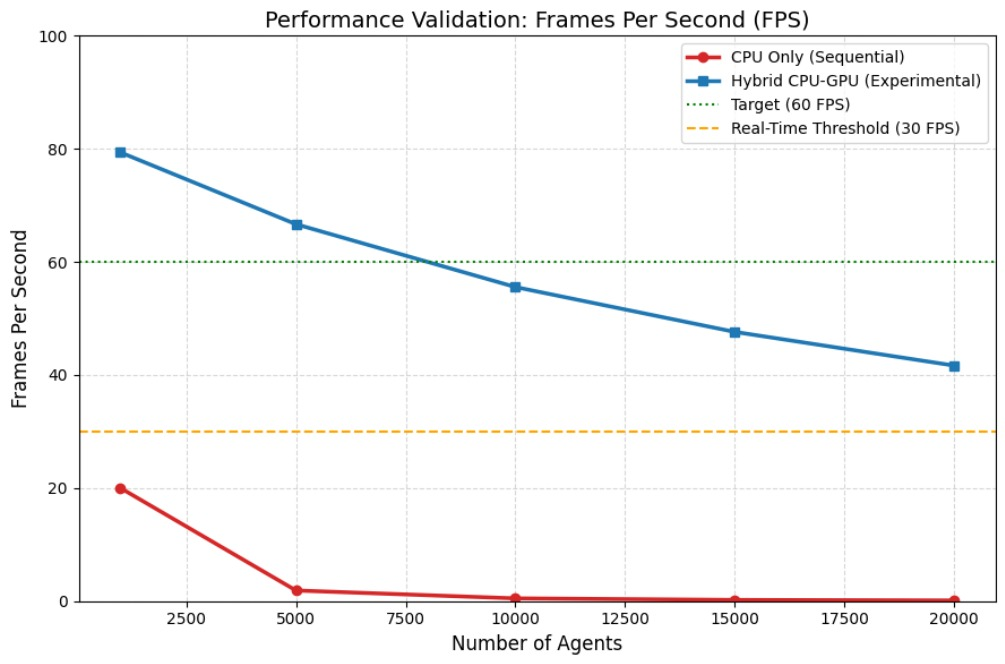
\includegraphics[width=0.8\textwidth]{image_95f261.jpeg}
    \caption{FPS Comparison: CPU Only vs. Hybrid CPU-GPU}
    \label{fig:fps_comp}
\end{figure}

As illustrated in Figure \ref{fig:fps_comp} the Hybrid CPU-GPU architecture maintains an experimental performance of 55.6 FPS at 10,000 agents, remaining well above the 30 FPS real-time threshold. In contrast, the CPU Only implementation fails to remain functional, crashing to near 0 FPS as the population scales.

\section{Execution Time and Scalability}
The reduction in computation time per simulation step is the direct result of the parallel execution of boid updates.

\begin{figure}[h]
    \centering
    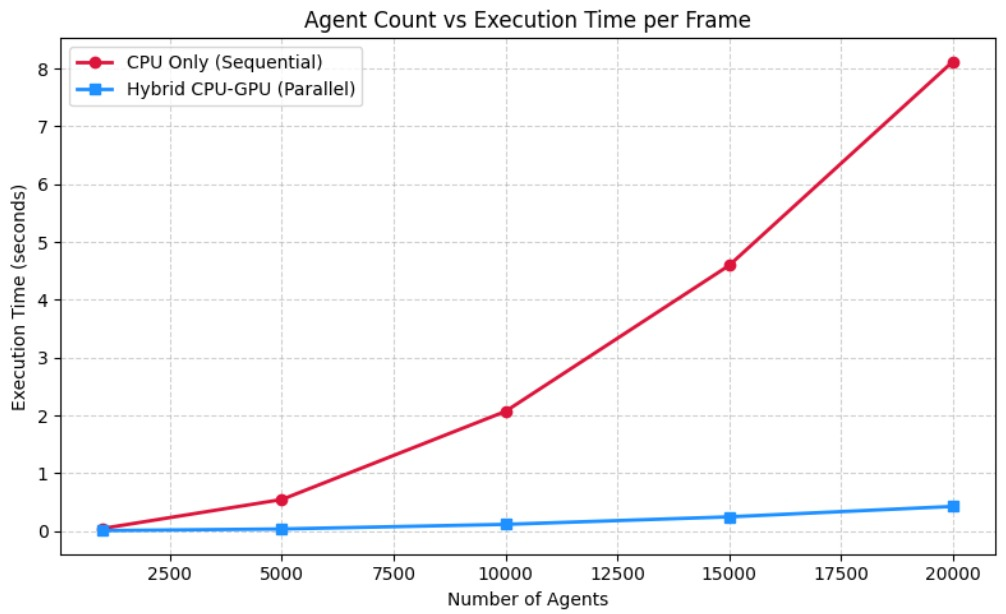
\includegraphics[width=0.8\textwidth]{image_95ef3a.jpeg}
    \caption{Agent Count vs. Execution Time per Frame}
    \label{fig:exec_time}
\end{figure}

As shown in Figure \ref{fig:exec_time} the execution time for the CPU follows a steep quadratic curve, reaching over 8 seconds per frame at 20,000 agents. The Hybrid model maintains a near-linear growth, keeping the processing time under 0.5 seconds even at peak loads, confirming the system's scalability.

\section{Computational Throughput}
To further quantify the performance gains, we analyzed the computational throughput, defined as agents processed per second.

\begin{figure}[h]
    \centering
    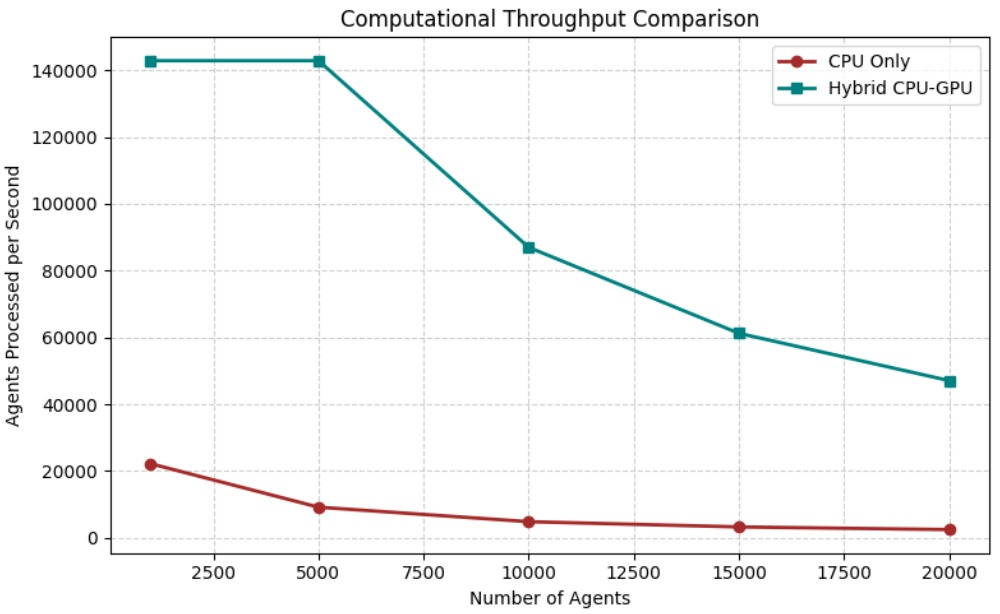
\includegraphics[width=0.8\textwidth]{image_95ef3f.jpeg}
    \caption{Computational Throughput Comparison}
    \label{fig:throughput}
\end{figure}

Figure \ref{fig:throughput} highlights a significant throughput gap. While the CPU's ability to process agents collapses under density, the Hybrid architecture processes approximately 20x to 40x more agents per second. This allows the simulation to capture complex behaviors like bottlenecking without visual stuttering.

\section{Behavioral Realism}
Beyond raw computational speed, the simulation effectively models authentic crowd dynamics:
\begin{itemize}
    \item \textbf{Bottleneck Formation}: Natural congestion is observed near designated exit points.
    \item \textbf{Lane Formation}: Agents develop organized flow patterns during high-speed movement.
    \item \textbf{Density-Based Heatmapping}: The use of color-coded agents (Green to Red) provides immediate visual feedback on areas of high crowd concentration.
\end{itemize}

The results confirm that the hybrid CPU–GPU architecture not only improves computational efficiency but also preserves the realism of crowd dynamics, making the system suitable for practical evacuation analysis.
%================ CONCLUSION =================%
\chapter{Conclusion}

This project demonstrates the effectiveness of hybrid CPU--GPU architectures in solving computationally intensive problems such as crowd simulation. By leveraging parallel computing principles, the system achieves scalability, efficiency, and real-time performance.

The proposed approach provides a robust framework for future research in large-scale simulations and highlights the importance of heterogeneous computing in modern applications.

%================ REFERENCES =================%
\begin{thebibliography}{9}

\bibitem{boids}
C. Reynolds, “Flocks, Herds, and Schools: A Distributed Behavioral Model,” 1987.

\bibitem{cuda}
D. Kirk and W. Hwu, Programming Massively Parallel Processors, 2016.

\end{thebibliography}

\end{document}